\section{Geolokalisierung} \label{sec:ueberblick} 

		Enthält ein Datensatz Informationen zu einem geografischen Objekt, so können in diesem geografische Indikatoren enthalten sein.
		Durch diese geografischen Indikatoren kann dem Datensatz, und damit dem geografischen Objekt, eine Georeferenz zugewiesen werden. 

		Die Zuordnung einer Georeferenz mit Hilfe von geografischen Indikatoren soll Geolokalisierung genannt werden.  

		In Abbildung \ref{img:geolokalisierung} wird dies dargestellt.
		Im Gegensatz zu Abbildung \ref{img:geogIndi} ist kein direkter Verweis vom geografischen Objekt zu einer Georeferenz vorhanden. 
		Stattdessen wird mit Hilfe der geografischen Indikatoren a und b durch die Geolokalisierung eine Georeferenz zugeordnet.

		\begin{figure}[!ht]
		\begin{center}
		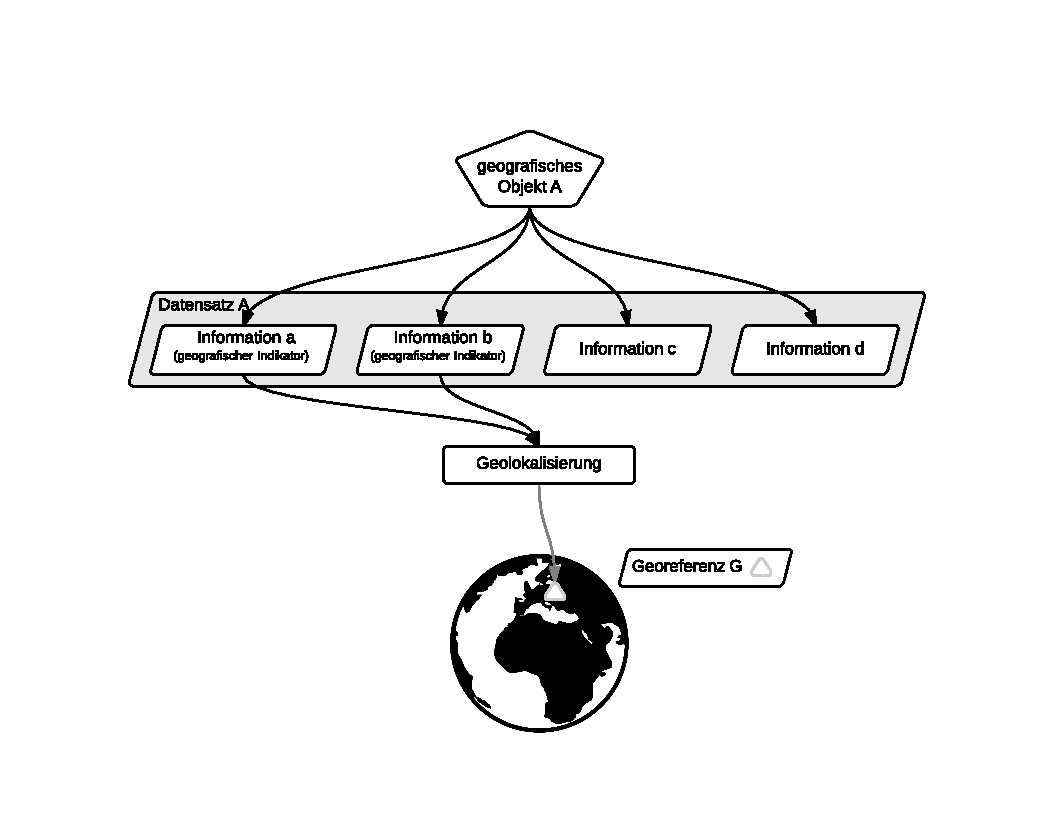
\includegraphics[scale=1.0]{geolokalisierung.pdf}
		\caption{Geografische Hierarchieebenen}
		\label{img:geolokalisierung}
		\end{center}
		\end{figure}	

		Um aus den geografischen Indikatoren eine Georeferenz ableiten zu können soll eine Datenbasis verwendet werden.
		Diese ordnet den geografischen Indikatoren eine Georeferenz zu.
		Die gespeicherte Georeferenz ist bekannt und kann genau bestimmt werden. 
		Das bedeutet: Ein Hinweis auf eine geografische Position wird auf eine konkrete, bekannte geografische Position abgebildet.
		Eine solche Datenbasis soll Georeferenz-Basis genannt werden.  

		Im einfachsten Fall liegt ein geografischer Indikator vor, dem direkt eine Georeferenz zugewiesen werden kann.
		Dies kann Beispielsweise ein eindeutiges Toponym sein.	
		Ein Ortsverzeichnis könnte hier als Georeferenz-Basis verwendet werden.
		Liegt der Datenwert "'Karlsruhe"' vor so würde die Geolokalisierung durch eine Abfrage an die Georeferenz-Basis die Stadt Karlsruhe als Georeferenz zuweisen.

		Wie in Kapitel \ref{sec:ToponymeInGeografischenIndikatoren} bereits erläutert sind Toponyme allerdings nicht immer eindeutig oder bekannt. 
		Die Abfrage an ein Ortsverzeichnis liefert potenziell mehrere Ergebnisse was eine weitere Verarbeitung der Ergebnisse erfordert.
		Ist das Toponym nicht bekannt so kann kein Ergebnis geliefert.

		Des weiteren sind die Datenwerte eines Datensatzes nicht immer direkt zu verwenden.
		Dies kommt ganz darauf an wie die Daten erhoben wurden. 
		Nutzereingaben auf Webseiten können beispielsweise aus einer Liste gewählt, oder in ein Freitext-Feld eingegeben werden.
		Werden die Datenwerte durch eine Liste erhoben liegt eine klar definierte Menge an möglichen Datenwerten vor.
		Haben die Datenwerte in der Liste geografischen Bezug so können ihnen Georeferenzen zugeordnet werden.
		Die so entstandenen Paare aus Datenwert und Georeferenz können in der Georeferenz-Basis abgespeichert werden.

		Soll ein Nutzer in ein Freitext-Feld seinen aktuellen Standort eingeben, und der Datenwert wird direkt übernommen muss dieser vorverarbeitet werden.
		Es ist zwar wahrscheinlich, dass der Nutzer ein Toponym angibt, aber es kann durch die direkte Übernahme der Eingabe zu Problemen kommen.
		Zunächst kann nicht einmal entschieden werden ob der Datenwert überhaupt einen geografischen Indikator darstellt.
		Zudem können in einem Freitext-Feld mehrere geografische Indikatoren auftauchen.
		Diese können widersprüchlich sein oder aber eine geografische Position genauer spezifizieren. 
		Durch die direkte Übernahme des Wertes können alle in Kapitel \ref{sec:ToponymeInGeografischenIndikatoren} aufgeführten Probleme auftreten.
		Dies macht die Zuordnung einer Georeferenz durch eine Ortsverzeichnis schwierig.
		Soll trotzdem mit Hilfe eines Ortsverzeichnisses eine Geolokalisierung durchgeführt werden ist zumindest eine umfangreiche Vor- und Nachverarbeitung nötig.

		In Abbildung \ref{img:geolokalisierungBsp} ist ein Beispiel zur Verwendung einer Georeferenz-Basis dargestellt.
		Der Datenwert "'Karlsruhe"' wird dabei auf eine Georeferenz aufgelöst indem eine Abfrage an die Georeferenz-Basis durchgeführt wird.
		Die zurückgelieferte Georeferenz wird dem Datensatz zugeordnet.

		\begin{figure}[!ht]
		\begin{center}
		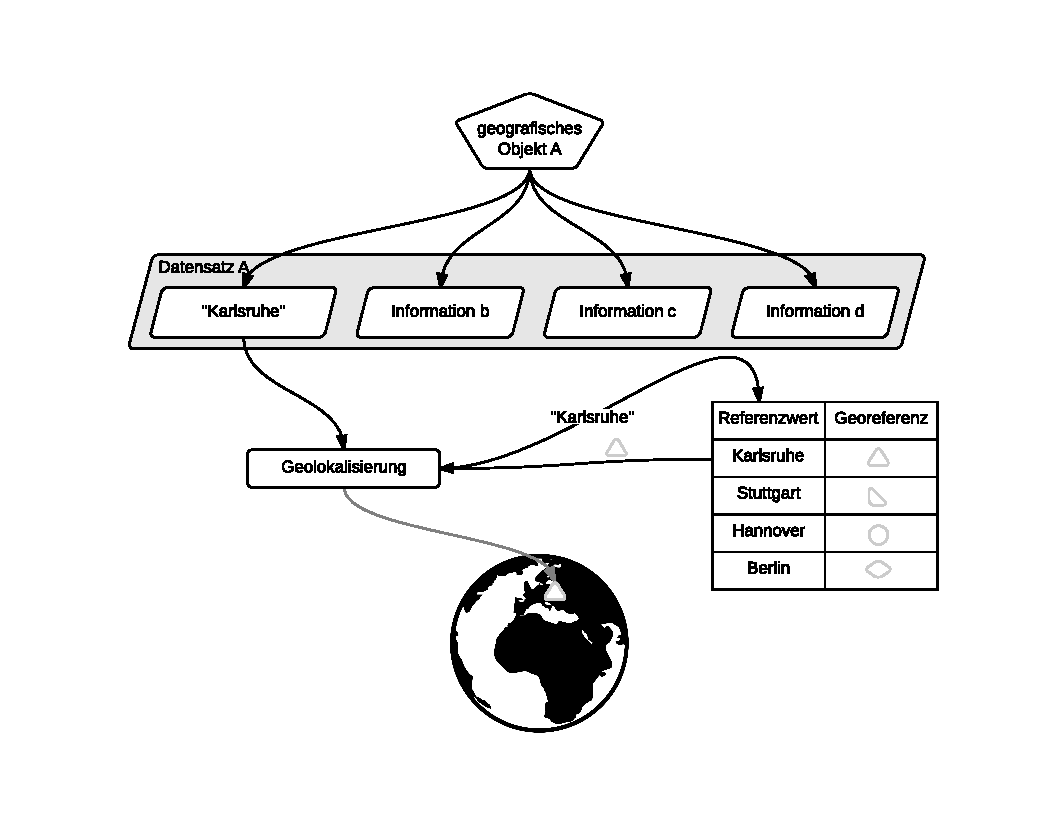
\includegraphics[scale=1.0]{geolokalisierungBsp.pdf}
		\caption{Geolokalisierung mit Referenz-Basis}
		\label{img:geolokalisierungBsp}
		\end{center}
		\end{figure}	

		Im folgenden Kapitel soll eine erste Struktur für eine Georeferenz-Basis vorgestellt werden.
		Es sollen dabei die minimalen Anforderungen an eine solche Datenbasis erfüllt werden.

	\section{Minimale Struktur einer Georeferenz-Basis zur Geolokalisierung} \label{sec:generelleStruktur} 
		
		Nach Abbildung \ref{img:geolokalisierung} wird bei der Geolokalisierung einem oder mehreren geografischen Indikatoren eine Georeferenz zugewiesen.
		In der einfachsten Variante wird lediglich ein einziger geografischer Indikator an die Geolokalisierung übergeben, und genau eine Georeferenz zurückgegeben.
		Die Geolokalisierung muss also zu einem gegebenen geografischen Indikator eine Georeferenz bestimmen können.
		Dies führt zu einer ersten einfachen Struktur für die Georeferenz-Basis.	

		Es wird angenommen der geografische Indikator stellt immer ein eindeutiges Toponym dar.
		Des weiteren sind alle möglichen Toponyme sowie eine zugehörige Georeferenz bekannt. 
		Die Georeferenz liegt als Adresse mit Straße, Hausnummer, Postleitzahl und Ortsname vor.

		Jedem möglichen Toponym soll eine Georeferenz zugeordnet werden können. 
		Die Georeferenz-Basis muss also eine Menge von Toponymen und zugehörigen Georeferenzen beinhalten
		Dieser Aufbau entspricht einer Art Wörterbuch in dem Informationen zu einem gegebenen Referenzwert nachgeschlagen werden können.
		Im vorliegenden Fall kann also zu einem Toponym die entsprechende Georeferenz nachgeschlagen werden.
		Die Referenzwerte stellen dabei mögliche Werte für den geografischen Indikator dar. 
		In Abbildung \ref{tab:simpleStruktur} ist ein Beispiel für eine sehr simple Struktur dargestellt.

		\begin{table}[htpb]
				\caption{Beispiel für eine Georeferenz-Basis} 
				\centering
				\begin{tabular}{|c||c|}
					\hline
					Referenzwert & Georeferenz \\
					\hline\hline
					Zoo-Karlsruhe & Ettlinger Straße 6 - 76137 Karlsruhe \\
					\hline
					ZKM & Lorenzstraße 19 D - 76135 Karlsruhe \\
					\hline
					Elbphilharmonie & Dammtorwall 46 - 20355 Hamburg \\
					\hline
				\end{tabular}
				\label{tab:simpleStruktur} 
		\end{table} 

		Wird eine Abfrage auf die Georeferenz-Basis mit den geografischen Indikatoren "'Zoo-Karlsruhe"', "'ZKM"' oder "'Elbphilharmonie"' durchgeführt, kann nun eine Georeferenz zurückgeliefert werden.
		Diese simple Struktur reicht grundsätzlich aus um eine Geolokalisierung durchführen zu können.
		In dem angeführten Beispiel ist die Menge der möglichen Toponyme sehr begrenzt, aber diese kann beliebig erweitert werden.
		Damit können sehr mächtige Datenbanken erstellt werden.

		Die meisten Ortsverzeichnisse sind nach dieser Struktur aufgebaut, wenngleich sie neben der Georeferenz noch andere Informationen zu einem Toponym liefern.

		Die Form in der die Georeferenz angegeben wird ist abhängig von der Anwendung. 
		Im Beispiel \ref{tab:simpleStruktur} wurden Adressen verwendet. 
		Dazu muss das angegebene Toponym oder die Zeichenkette jedoch eine Adresse besitzen. 
		Ein See in der Wildnis Alaskas wird keine solche Adresse aufweisen.
		Aber auch die geografische Position einer Stadt oder eines Landes kann nicht durch eine Adresse beschrieben werden. 
		Die Form in der die Georeferenz angegeben wird kommt auf den jeweiligen Anwendungsfall an.
		
		\subparagraph{Mögliche Angaben für die Georeferenz}

		\begin{itemize}
		  	 \item geografische Koordinaten
		  	 \item vollständige Adressen
		  	 \item Ländernamen
		  	 \item Städtename
		  	 \item Namen für Verwaltungseinheiten 
		  	 \item Zeitzonen
		  	 \item Straßenname und Kilometerangabe
		  	 \item ...
		  \end{itemize}  

	 	Grundsätzlich sind alle Formen, welche eine direkte oder indirekte Georeferenz darstellen, denkbar.
	 	Die Angabe muss lediglich die gegebenen Anforderungen an die Geolokalisierung erfüllen.

	  	Für den Straßenverkehr ist eine Angabe einer Adresse ausreichend.
		Für Wanderungen in unerschlossenen Gebieten hingegen sind geografische Koordinaten notwendig. 

		Wie in der Liste zu erkennen ist kann die Georeferenz auch als Toponym angegeben werden.
		Wenn nun ein Toponym abgefragt wird, wird als Georeferenz ein Toponym zurückgeliefert.
		Dies macht auf den ersten Blick wenig Sinn.
		Die geografischen Indikatoren sind jedoch vorerst nur Hinweise auf eine Georeferenz.
		Liefert eine Georeferenz-Basis ein Ergebnis zurück, ist der geografische Bezug bestätigt und dem Datensatz kann eine bekannte Georeferenz zugeordnet werden.				
	
	

	

----------------------->>>>>>>>>>>>>
			

		\subsection{Vorverarbeitung des Nutzer-Standortes und der Nutzer-Zeitzone} \label{subsec:VorverarbeitungStandortZeitzone} 
			
			Es ist zunächst nötig die genutzten geografischen Indikatoren einer Vorverarbeitung zu unterziehen. 
			Ziel ist es aus dem Nutzer-Standort möglichst viele Informationen zu extrahieren und etwaige Probleme zu beseitigen.
			In der folgenden Liste sind einige Nutzer-Standorte angegeben. 
			Anhand dieser Liste sollen die Vorverarbeitungsschritte demonstriert werden.

			\begin{multicols}{2}
			\begin{enumerate}
				\item Bélem-PA
				\item West Sussex, England
				\item South Florida
				\item Pitmedden,  Scotland, UK
				\item Mato Grosso \& Rio de Janeiro
				\item -****-
				\item USA \textbackslash/ Los Angeles
				\item Nottingham\textbackslash/London
				\item Los Angeles, USA
				\item I $\heartsuit$ New York 
				\item $\dagger$\textasciitilde Los Angeles\textasciitilde$\dagger$
				\item earth-sea
				\item In front of the computer
				\item 11th Dimension | California
				\item York
				\item York
			\end{enumerate}
			\end{multicols}
				
			

			

			

			

			
			\subsubsection{Fazit} 

				Nach der Vorverarbeitung liegen eine Menge von potenziellen geografischen Indikatoren mit zugehörigen geografischen Koordinaten vor.
				Bei der Vorverarbeitung wurden einige Probleme des Nutzer-Standortes beseitigt.
				Insbesondere können Datenwerte separat voneinander betrachtet werden.

				Die so erzeugten potenziellen geografischen Indikatoren können nun in der Georeferenz-Basis als Referenzwerte gespeichert werden.
				Mit der so erzeugten Georeferenz-Basis ist es grundsätzlich möglich eine Geolokalisierung durchzuführen. 
				Allerdings wird jedem potenziellen geografischen Indikator eine Georeferenz zugeordnet.
				Das ist grundsätzlich problematisch, da Referenzwerten die keinen geografischen Bezug aufweisen eine Georeferenz zugeordnet wird. 
				Dies kann bei der Geolokalisierung zu Fehlern führen.
				Ein Referenzwert mit geografischem Bezug wird gleich behandelt wie ein Referenzwert ohne geografischen Bezug.
				Es sollte entschieden werden können ob der Referenzwert einen geografischen Bezug hat oder nicht.
				Bisher existiert noch kein Hinweis auf den geografischen Bezug.
				Es existiert lediglich eine Datenbasis die Referenzwerten eine Georeferenz zuweist. 

				Des weiteren können zu einem Referenzwert beliebig viele Datensätze existieren, selbst wenn diese auf denselben Ort verweisen. 
				Bei einer Abfrage an die Datenbank werden potenziell große Mengen an Datensätzen zurückgeliefert die alle auf dieselbe Georeferenz verweisen.

		

		

		\subsection{Erweiterte Struktur der Georeferenz-Basis} \label{subsec:erweiterteStruktur} 

			Hier soll nun die erweiterte Struktur der Georeferenz-Basis vorgestellt werden.
			Mit der absoluten Häufigkeit ist ein neuer Wert pro Datensatz hinzugekommen.
			Des weiteren wurde die Georeferenz auf eine Stadt aufgelöst und damit implizit die Verwaltungseinheit erster Ordnung (Adm1), die Verwaltungseinheit zweiter Ordnung (Adm2) und das Land mitbestimmt. 
			Diese sollen nun zusätzlich in der Struktur hinterlegt werden.
			Die daraus resultierende Struktur der Georeferenz-Basis ist in \ref{tab:strukturMitHierarchie1} inklusive einiger Beispieleinträge dargestellt.


			\begin{table}[htpb]
				\caption{Struktur der Georeferenz-Basis mit geografischer Hierarchie} 
				\centering
				\tiny
				\begin{tabular}{|c|c|c|c|c|c|}
					\hline
					Referenzwert & Stadt & Adm2 & Adm1 & Land & abs. Häufigkeit \\
					\hline\hline
					 Los+Angeles    USA   & Los Angeles & LA County & CA & USA & 30 \\
					\hline
					 Los+Angeles    USA   & San Francisco & SF County & CA & USA & 3 \\
					\hline
					 Los+Angeles   & Los Angeles & LA County & CA & USA & 70 \\
					\hline
					 USA   & Los Angeles & LA County & CA & USA & 80 \\
					\hline
					 Heilbronn   & Heilbronn & Regierungsbezik Stuttgart & BaWü & BRD & 90\\
					\hline
				\end{tabular}
				\label{tab:strukturMitHierarchie1} 
			\end{table} 

		\subsection{Überblick}

			Hier soll nun ein Überblick über das gesamte Verfahren zum einlernen der Georeferenz-Basis gegeben werden.

			In Abbildung \ref{img:einlernenAblauf} ist der Gesamtablauf des Einlernens dargestellt.  
			Zunächst werden die einzelnen Vorverarbeitungsschritte für den Nutzer-Standort und die Nutzer-Zeitzone durchgeführt.
			Parallel kann der Längen- und Breitengrad auf eine Stadt aufgelöst werden.
			Die dadurch entstandenen potenziellen geografischen Indikatoren und die zugehörige Georeferenz wird nun in die Georeferenz-Basis gespeichert. 
			Dabei wird überprüft ob dieser Datensatz bereits vorhanden ist. 
			Ist dies der Fall, wird der Häufigkeitswert des entsprechenden Datensatzes inkrementiert.
			Ist der Datensatz noch nicht vorhanden wird er angelegt und die absolute Häufigkeiten mit 1 initialisiert.

			 \begin{figure}[!ht]
					\begin{center}
						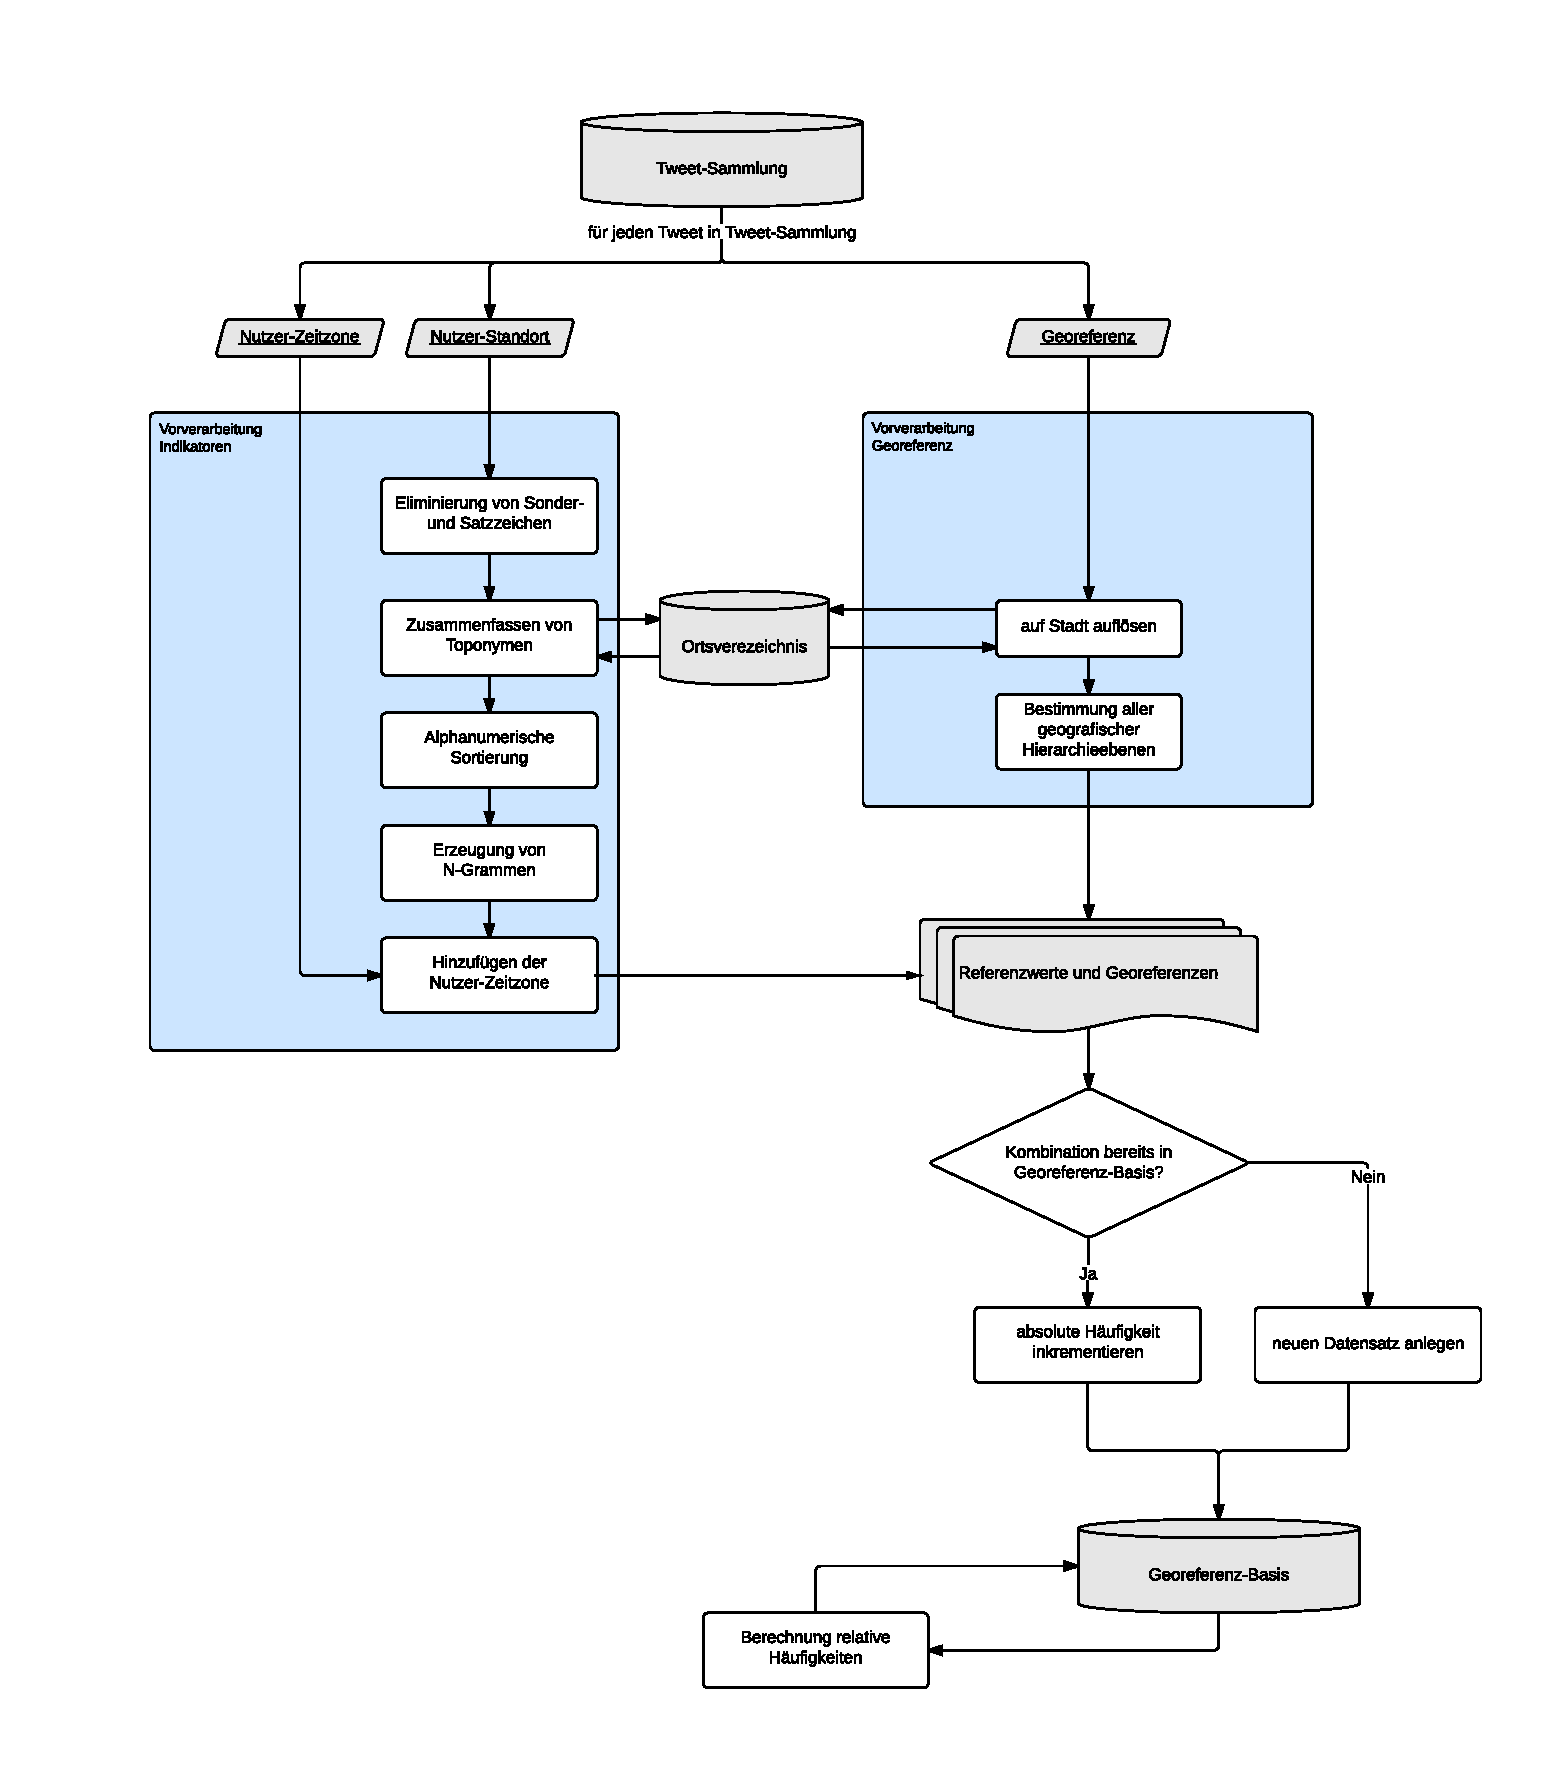
\includegraphics[scale=0.6]{einlernenAblauf.pdf}
						\caption{Ablaufplan einlernen}
						\label{img:einlernenAblauf}
					\end{center}
				\end{figure}


			Die Vorverarbeitung extrahiert dabei zusätzliche Informationen aus dem Nutzer-Standort.
			Durch die Bereiningung der Werte im Nutzer-Standort, die alphanumerische Sortierung, das identifzieren von Toponymen mit mehreren Worten und die darauffolgende Erzeugung von N-Grammen werden zusätzliche Informationen aus jedem Nutzer-Standort gewonnen.
			Die Nutzer-Zeitzone wird einbezogen um Doppeldeutigkeiten auflösen zu können.

			Durch die neue Datenstruktur, mit den absoluten Häufigkeiten und der abgebildeten geografischen Hierarchie, lassen sich nun tiefergehende Analysen durchführen um eine robuste Geolokalisierung zu ermöglichen. 
			Die absoluten Häufigkeiten geben dabei an wie oft ein Referenzwert in einer bestimmten Region vorkommt.

			Durch dieses Verfahren lässt sich eine Datenbasis erzeugen die domänenspezifische Eigenheiten, in Bezug auf die Verwendung spezieller Begriffe oder Formulierungen, berücksichtigt.
			Des weiteren werden Toponyme, die in Ortsverzeichnissen unter Umständen nicht hinterlegt sind, berücksichtigt.
			Auch geografische Indikatoren mit mittelbarem geografischen Bezug, zum Beispiel die Verwendung spezieller Begriffe in einer geografischen Region, können einbezogen werden. 

	\section{Geografischer Bezug der eingelernten Referenzwerte} \label{sec:geografischerBezug} 
			
		Die eingelernten Referenzwerte beinhalten alle Werte aus den Nutzer-Standorten der Tweet-Lerndaten.
		Es sind also auch Referenzwerte vorhanden die keinen geografischen Bezug haben.
		Es ist die Frage zu beantworten: Wie kann bestimmt werden ob ein Referenzwert geografischen Bezug hat oder nicht?
		Oder: Wie kann vermieden werden, dass ein Referenzwert, der keinen geografischen Bezug hat, zur Geolokalisierung genutzt wird?
		
		Dies ist wichtig, denn durch die Referenzwerte wird in der eigentlichen Geolokalisierung einem geografischen Indikator eine Georeferenz zugewiesen. 
		Wird einem geografischen Indikator durch einen Referenzwert ohne geografischen Bezug eine Georeferenz zugewiesen ist diese mit hoher Wahrscheinlichkeit fehlerhaft.
		Dies wiederum führt zu schlechten und unzuverlässigen Ergebnissen.
		Es muss also ein Verfahren gefunden werden um zu entscheiden ob die Referenzwerte einen geografischen Bezug haben oder nicht.

		Es ist zu beachten, dass die Vorverarbeitung keine Aussage zum geografischen Bezug macht, sondern vielmehr die Referenzwerte aus den Nutzer-Standorten extrahiert. 
		Dies soll sicherstellen, das möglichst viele Informationen aus den Nutzer-Standorten gezogen werden können und insbesondere keine Informationen verloren gehen.  
		
		Um zu entscheiden ob ein Referenzwert geografischen Bezug hat oder nicht wird die absolute Häufigkeit verwendet.
		Die absoluten Häufigkeiten geben an wie oft ein Referenzwert in einer bestimmten Region, zunächst in der Voronoi-Region der entsprechenden Stadt, vorkommt.			 
		Daraus kann nun ein geografischer Bezug abgeleitet werden.

			 



		\subsection{Analyse}

			Die Analyse beinhaltet zwei Schritte. 
			Zuerst müssen diejenigen Referenzwerte gewählt werden, welche am wahrscheinlichsten einen geografischen Bezug haben.
			Dabei wird jeder Referenzwert separat betrachtet. 
			In einem nächsten Schritt wird derjenige Referenzwert gewählt, der unter den verbliebenen am wahrscheinlichsten die geografische Position des Nutzers beschreibt. 

			\subsubsection{Auswahl der Referenzwerte mit geografischem Bezug}

				Es können pro Referenzwert zunächst mehrere Datensätze vorliegen.
				Aus diesen sollen diejenigen gewählt werden, welche am wahrscheinlichsten einen geografischen Bezug aufweisen.
				Dazu werden sowohl die absoluten als auch die relativen Häufigkeiten genutzt. 
				Für jeden Referenzwert wird derjenige Datensatz gewählt, der die größte relative Häufigkeit $h_{rel}$ über einem Schwellwert $s_{rel}$ aufweist.
				Mit diesem Schwellwert lässt sich bestimmen wie verteilt der Referenzwert auftreten kann.
				Zusätzlich wird geprüft ob die absolute Häufigkeit ebenfalls über einem Schwellwert $s_{abs}$ liegt.
				Mit diesem Schwellwert lässt sich bestimmen wie häufig der Referenzwert an einer geografischen Position oder in einer geografischen Region auftreten muss. 

			\subsubsection{Bestimmung der wahrscheinlichsten Georeferenz} 

				Nun liegt wiederum eine Menge an Datensätzen vor.
				Jeder Referenzwert, und damit auch jeder potenzielle geografische Indikator, taucht nur noch ein mal auf. 

				Aus den verbliebenen Datensätzen soll nun die Georeferenz gewählt werden. 
				Dazu werden die relativen Häufigkeiten verglichen.
				Es wird der Datensatz mit der höchsten relativen Häufigkeit gewählt.
				Die Georeferenz dieses Datensatzes wird dann dem Twitter-Nutzer zugewiesen. 
				Damit wird der Referenzwert ausgewählt der die größte relative Häufigkeit aller untersuchten Referenzwerte aufweist. 

				Die Referenzwerte stellen NGramme dar, wie in der Vorverarbeitung in Unterkapitel \ref{subsec:VorverarbeitungStandortZeitzone} erläutert wird.
				Es werden hier also insbesondere auch Uni-, Bi- und Trigramme miteinander verglichen.
				Darauf soll nun eingegangen werden.

				\paragraph{Vergleich der relativen Häufigkeiten zu Uni- Bi- und Trigrammen}

					Jedes Element eines Bi- oder Trigrammes kann potenziell einen geografischen Bezug haben. 
					Umso mehr Elemente ein NGramm beinhaltet umso spezieller kann die Beschreibung des geografischen Objekts sein.
					Deshalb können NGramme mit einem höheren Grad ein Objekt genauer beschreiben als NGramme mit einem niedrigeren Grad.

					Allerdings können NGramme mit einem höheren Grad auch eine schlechtere Beschreibung darstellen. 
					Beispielsweise wenn das zusätzliche Element keinen geografsichen Bezug hat.

					Bei NGrammen mit einem Grad größer zwei können also zwei Fälle unterschieden werden.

					\begin{enumerate}
						\item Die Kombination aus den Elementen des NGrammes beschreibt einen Ort genauer
						\item Die Kombination aus den Elementen des NGrammes beschreibt einen Ort nicht genauer
					\end{enumerate}

					\subparagraph{Fall1} 

						Ein Beispiel für den ersten Fall ist der Nutzer-Standort "'york"' mit der Nutzer-Zeitzone "'eastern+time+us+canada"'. 
						Durch die Vorverarbeitung werden folgende potenzielle geografische Indikatoren erzeugt.
						\begin{enumerate}		
							\item york
							\item york \textit{eastern+time+us+canada}
						\end{enumerate}		

						Eine Stadt Namens York existiert sowohl in Grossbritannien als auch in den USA.
						Fragt man nun die beiden Referenzwerte in der Georeferenz-Basis ab erhält man folgende Werte:

							\begin{table}[h]
								\centering
									\caption{"'york"'}
									\label{tab:york}
									\begin{tabular}{|l|l|l|l|}
									\hline
									Referenzwert 				& Stadt  	& abs. Häufigkeit & rel. Häufigkeit in \% \\ \hline \hline
									York          				& York (GB) & 97              & 48,3       \\ \hline
									york eastern+time+us+canada & York (US) & 12              & 63,2        \\ \hline
									\end{tabular}
							\end{table}

							Die realtive Häufigkeit für york in Kombination mit der Zeitzone ist höher. 
							Die Zeitzone gibt zusätzliche Auskunft darüber welches York gemeint ist. 
							Die Kombination ist spezieller, kommt deshalb seltener vor und potenziell eher dort wo sie zutrifft. 
							In diesem Fall in York in den USA. 

							In den meisten Fällen beschreibt einer der beiden Indikatoren eine größere geografische Region wie beispielsweise einen Bundesstaat der USA.
							Wird ein weiterer Wert, beispielsweise ein Städtename hinzugenommen, wird die Angabe des Ortes genauer. 
							Die Wahrscheinlichkeit, dass diese Kombination ausserhalb des Ortes auftritt wird geringer. 

					\subparagraph{Fall 2}

						Hier können wiederum 2 Fälle unterschieden werden.

						\begin{enumerate}
							\item Beide Elemente beziehen sich auf unterschiedliche geografische Objekte
							\item Nur ein Element hat geografischen Bezug das andere nicht 
						\end{enumerate}

						Wenn zu einem Referenzwert mit geografischem Bezug ein Element hinzugefügt wird, welches keinen geografischen Bezug hat, beschreibt dies den Ort nicht genauer.
						Es ist zu erwarten, dass die Kombination der Elemente sehr selten vorkommt oder sehr verteilt ist. 
						Ist die Kombination verteilter, so ist der relative Wert geringer als der des einzelnen Referenzwertes mit geografischem Bezug.
						Ist die Kombination seltener kann der Referenzwert bereits durch den Schwellwert $s_{abs}$ aussortiert werden.		

						Wenn zu einem Referenzwert mit geografischem Bezug ein Element hinzugefügt wird, welches zwar geografischen Bezug hat, aber dieses sich auf ein anderes geografisches Objekt bezieht ist dasselbe Verhalten zu erwarten.
						
			